%%%%%%%%%%%%%%%%%%%%%%%%%%%%%%%%%%%%%%%%%
%%% HYPERRIDE Reporting Template
%%%%%%%%%%%%%%%%%%%%%%%%%%%%%%%%%%%%%%%%%

\documentclass[letterpaper,12pt]{report}
\usepackage[pass]{geometry}
\usepackage{istgame}
\usepackage{xcolor}
\usepackage{xurl}
\usepackage{hyperride}		% HYPERRIDE specific definitions and styles  
\usepackage[utf8]{inputenc}	% UTF8 package
\usepackage[T1]{fontenc}
\usepackage{textcomp}		% common special chars
\usepackage{amsmath}		% math formula
\usepackage{fancybox}
\usepackage{anyfontsize}	% fonts
\usepackage{lipsum}
\usepackage{float}
\usepackage[normalem]{ulem}
\usepackage{cleveref}
\usepackage[printonlyused]{acronym}
\hypersetup{
	pdftitle={Beacon Labs - Workshop},
	pdfauthor={[Dylan Gresham, Jordan Whyte, Gunnar Vittrup, Josh Boyle, Gaby Dagher]},
	pdfkeywords={Beacon Labs, Workshop, Cybersecurity, Middlebox, TCP Amplification, Network Security, Mobile Security, Web Security, Service Workers, XSS, Cross-Site Scripting, Android Vulnerability},
}
\usepackage{booktabs}
\usepackage{subfigure}
\usepackage{graphicx}
\usepackage{xcolor}
\usepackage{soul}
\sethlcolor{lightgray}
\usepackage[export]{adjustbox}
\usepackage{mdframed}
\usepackage{pdfpages}
\usepackage{comment}
\usepackage{multirow,array}
\def\todo#1{{\color{hyperridered}\textbf{TODO:} ``#1''}}
\def\hyperride{HYPERRIDE}
\definecolor{lightblue}{rgb}{0.87, 0.94, 1}
\graphicspath{ {graphics/} }

%%%%%%%%%%%%%%%%%%%%%%%%%%%%%%%%%%%%%%%%%
%%% Definitions
%%%%%%%%%%%%%%%%%%%%%%%%%%%%%%%%%%%%%%%%%

%% stuff for displaying code

% Define the listing package
\usepackage{listings} % code highlighter
\usepackage{color} % use color
\definecolor{mygreen}{rgb}{0,0.6,0}
\definecolor{mygray}{rgb}{0.5,0.5,0.5}
\definecolor{mymauve}{rgb}{0.58,0,0.82}

% Customize a bit the look
\lstset{ %
  backgroundcolor=\color{white}, % choose the background color; you must add \usepackage{color} or \usepackage{xcolor}
  basicstyle=\footnotesize, % the size of the fonts that are used for the code
  breakatwhitespace=false, % sets if automatic breaks should only happen at whitespace
  breaklines=true, % sets automatic line breaking
  captionpos=b, % sets the caption-position to bottom
  commentstyle=\color{mygreen}, % comment style
  deletekeywords={...}, % if you want to delete keywords from the given language
  escapeinside={\%*}{*)}, % if you want to add LaTeX within your code
  extendedchars=true, % lets you use non-ASCII characters; for 8-bits encodings only, does not work with UTF-8
  frame=tblr, % adds a frame around the code with line numbers inside the box
  keepspaces=true, % keeps spaces in text, useful for keeping indentation of code (possibly needs columns=flexible)
  keywordstyle=\color{blue}, % keyword style
  % language=Octave, % the language of the code
  morekeywords={*,...}, % if you want to add more keywords to the set
  numbers=left, % where to put the line-numbers; possible values are (none, left, right)
  numbersep=5pt, % how far the line-numbers are from the code
  numberstyle=\tiny\color{mygray}, % the style that is used for the line-numbers
  rulecolor=\color{black}, % if not set, the frame-color may be changed on line-breaks within not-black text (e.g. comments (green here))
  showspaces=false, % show spaces everywhere adding particular underscores; it overrides 'showstringspaces'
  showstringspaces=false, % underline spaces within strings only
  showtabs=false, % show tabs within strings adding particular underscores
  stepnumber=1, % the step between two line-numbers. If it's 1, each line will be numbered
  stringstyle=\color{mymauve}, % string literal style
  tabsize=2, % sets default tabsize to 2 spaces
  title=\lstname % show the filename of files included with \lstinputlisting; also try caption instead of title
}
% END of listing package %

\definecolor{darkgray}{rgb}{.4,.4,.4}
\definecolor{purple}{rgb}{0.65, 0.12, 0.82}

% Define Javascript language
\lstdefinelanguage{JavaScript}{
  keywords={typeof, new, true, false, catch, function, return, null, catch, switch, var, if, in, while, do, else, case, break},
  keywordstyle=\color{blue}\bfseries,
  ndkeywords={class, export, boolean, throw, implements, import, this},
  ndkeywordstyle=\color{darkgray}\bfseries,
  identifierstyle=\color{black},
  sensitive=false,
  comment=[l]{//},
  morecomment=[s]{/*}{*/},
  commentstyle=\color{purple}\ttfamily,
  stringstyle=\color{red}\ttfamily,
  morestring=[b]',
  morestring=[b]"
}

\lstset{
  language=JavaScript,
  extendedchars=true,
  basicstyle=\footnotesize\ttfamily,
  showstringspaces=false,
  showspaces=false,
  numbers=left,
  numberstyle=\footnotesize,
  numbersep=9pt,
  tabsize=2,
  breaklines=true,
  showtabs=false,
  captionpos=b
}

%%%%%%%%%%%%%%%%%%%%%%%%%%%%%%%%%%%%%%%%%
%%% Definitions
%%%%%%%%%%%%%%%%%%%%%%%%%%%%%%%%%%%%%%%%%
\newcounter{taskset}
\setcounter{taskset}{1} % Set the initial value of the taskset counter

\newcounter{action}[taskset]
\renewcommand{\theaction}{\thesection.\arabic{taskset}.\arabic{action}}

\newcommand{\myaction}[1]{%
  \refstepcounter{action}%
  \textbf{Action \theaction: #1}%
}


% CHANGE %'s below to make subsection headings visible/invisible in TOC
%\newcommand{\xsubsubsection}[1]{\subsection{#1}}
%\newcommand{\xsubsubsection}[1]{\subsubsection{#1}}

\setcounter{secnumdepth}{4}
\setcounter{tocdepth}{5}

\begin{document}


\includepdf[pages=1]{./graphics/2FP.pdf}

\mdfdefinestyle{code}{%
    linecolor=black,
    outerlinewidth=2pt,
    %roundcorner=20pt,
    innertopmargin=4pt,
    innerbottommargin=4pt,
    innerrightmargin=4pt,
    innerleftmargin=4pt,
    leftmargin = 4pt,
    rightmargin = 4pt
    backgroundcolor=black!10
}

\setcounter{tocdepth}{4}
\setcounter{secnumdepth}{4}

%%%%%%%%%%%%%%%%%%%%%%%%%%%%%%%%%%%%%%%%%
%%% URL style same as regular text
%%%%%%%%%%%%%%%%%%%%%%%%%%%%%%%%%%%%%%%%%
	
\urlstyle{same}

%%%%%%%%%%%%%%%%%%%%%%%%%%%%%%%%%%%%%%%%%
%%% Deliverable Information
%%%%%%%%%%%%%%%%%%%%%%%%%%%%%%%%%%%%%%%%%

% Project Meta Information
\ProjectFullTitle{Beacon Network Security Labs: Middlebox Amplification Attack Activity}
\ProjectAcronym{HYPERRIDE}
\ProjectRefNo{957788}

% Report Number, use either "1", "2", or "3" for the corresponding reporting period
\delivNumber{0}

% Period covered by the report
\delivFrom{dd/mm/yyyy}
\delivTo{dd/mm/yyyy}

% Report Responsible Partner
\delivResponsible{AIT Austrian Institute of Technology (AIT)} 

% Report Version, Contractual and Actual Date, Dissemination Level, Type
\delivVersion{vn.n}
\ContractualDate{dd/mm/yyyy}
\ActualDate{dd/mm/yyyy}

% List of Main Authors (usually from the responsible partner)
\delivAuthor{[Dylan Gresham, Gaby Dagher]}

% List of Co-Authors (all other co-authors should be listed here)
\delivFPAuthor{[]}

% Report Status
\delivStatus{d} %% d = draft, f = final, s = submitted

%%%%%%%%%%%%%%%%%%%%%%%%%%%%%%%%%%%%%%%%%
%%% Change Log
%%%%%%%%%%%%%%%%%%%%%%%%%%%%%%%%%%%%%%%%%

\istChange{dd/mm/yyyy}{v1.0}{Name (Partner short name)}{Draft report template}
\istChange{}{}{}{}

%%%%%%%%%%%%%%%%%%%%%%%%%%%%%%%%%%%%%%%%%
%%% Cover Page
%%%%%%%%%%%%%%%%%%%%%%%%%%%%%%%%%%%%%%%%%

%\makecover

%%%%%%%%%%%%%%%%%%%%%%%%%%%%%%%%%%%%%%%%%
%%% Table of Contents
%%%%%%%%%%%%%%%%%%%%%%%%%%%%%%%%%%%%%%%%%

\clearpage
\fancypagestyle{plain}{}
\settableofcontents
\tableofcontents
\clearpage

\newpage

%%%%%%%%%%%%%%%%%%%%%%%%%%%%%%%%%%%%%%%%%
%%% Setup
%%%%%%%%%%%%%%%%%%%%%%%%%%%%%%%%%%%%%%%%%

\section*{Setup}\label{sec:Setup}
\addcontentsline{toc}{section}{Setup}

\subsection*{Android Studio Installation}
\addcontentsline{toc}{subsection}{Android Studio Installation}

\paragraph*{Steps:}

\begin{enumerate}
    \item The latest versions of Android Studio have since deprecated the API version used in the workshop. To download a compatible version of Android Studio, open the \href{https://developer.android.com/studio/archive}{Android Studio Download Archive} (full link at the bottom of this step) and find ``Android Studio Ladybug Feature Drop | 2024.2.2 Patch 2'' from February 26, 2025. Expand the drop down to download an installer if you're on Windows or the zip archive if you're on Linux. For the Windows installer, the standard options will suffice. For Linux, after downloading and untarring the archive, cd into the untarred directory and then into the bin directory and run the \texttt{studio.sh} script to start Android Studio.

    \url{https://developer.android.com/studio/archive}
    \item Once the installation has finished, open Android Studio.
    \item The first time Android Studio is opened, it may prompt you to agree to their terms and conditions and install their SDKs, step through it for a standard installation if prompted.
    \item Once everything has finished downloading, move to the next section.
\end{enumerate}

\subsection*{Emulation Device Setup}
\addcontentsline{toc}{subsection}{Emulation Device Setup}

\paragraph*{Steps:}

\begin{enumerate}
    \item The device we'll be using for this activity is the Pixel 5 with API 28 (``Pie''). To start creating our emulation device, first download the activity starter code from \href{https://drive.google.com/file/d/17KuEH9aQtD4UuVXMFIOAWq97-_Z-CzXk/view?usp=sharing}{this Google Drive link}.
    
    \url{https://drive.google.com/file/d/17KuEH9aQtD4UuVXMFIOAWq97-_Z-CzXk/view?usp=sharing}
    \item Once downloaded, unzip into a directory.
    \item In Android Studio, choose the ``Open'' option (Figure~\ref{fig:android-open}) and open the directory where the activity materials were saved to. Depending on the tool used to unzip the project it may create a new directory with a subdirectory. Use the subdirectory as the directory to open (Figure~\ref{fig:android-open-project}).

    \begin{figure}[!htbp]
        \centering
        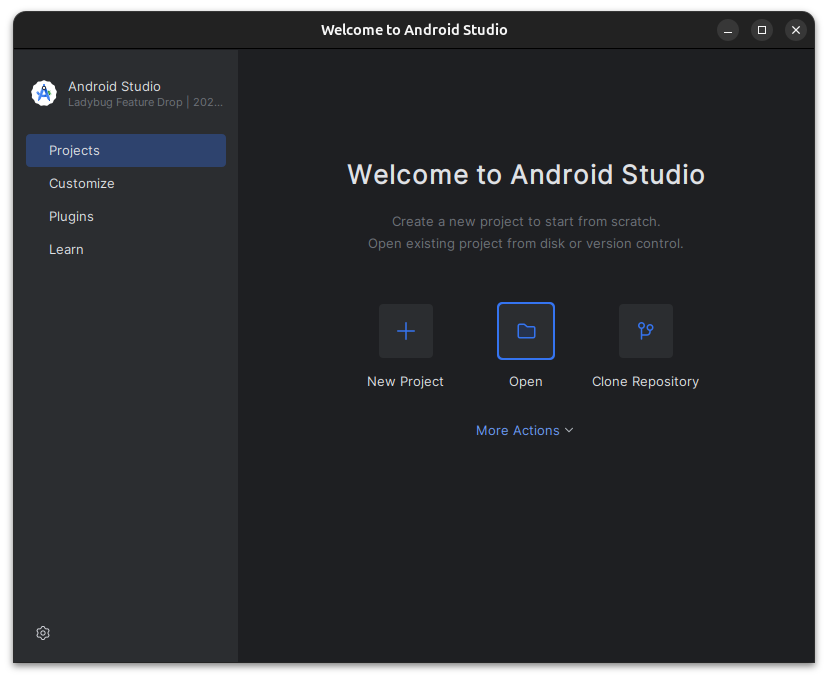
\includegraphics[width=0.5\linewidth]{graphics/studio-open.png}
        \caption{Android Studio open project}
        \label{fig:android-open}
    \end{figure}

    \begin{figure}[!htbp]
        \centering
        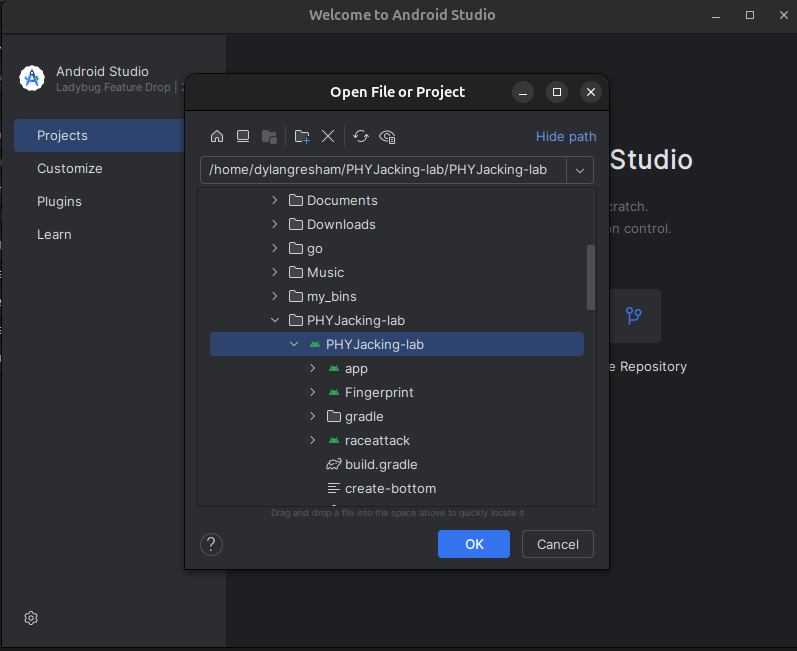
\includegraphics[width=0.75\linewidth]{graphics/studio-open-project.png}
        \caption{Android Studio open project file picker. Note that the selected directory is the direct parent of all of the source material, not the grandparent directory.}
        \label{fig:android-open-project}
    \end{figure}

    \item Once the project has been opened, navigate to the Device Manager (Figure~\ref{fig:device-manager}), click the ``+'' button and select the ``Create Virtual Device'' option.

    \begin{figure}[!htbp]
        \centering
        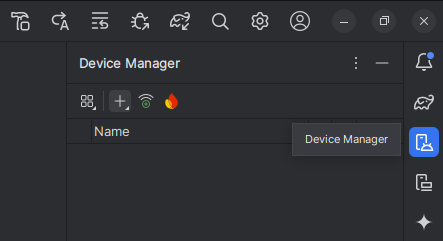
\includegraphics[width=0.75\linewidth]{graphics/studio-device-manager.png}
        \caption{Device Manager menu icon located on the right side of the IDE.}
        \label{fig:device-manager}
    \end{figure}
    
    \item Scroll down to or search for the ``Pixel 5'' device, select it and click Next (Figure~\ref{fig:pixel-5}).
    
    \begin{figure}[!htbp]
        \centering
        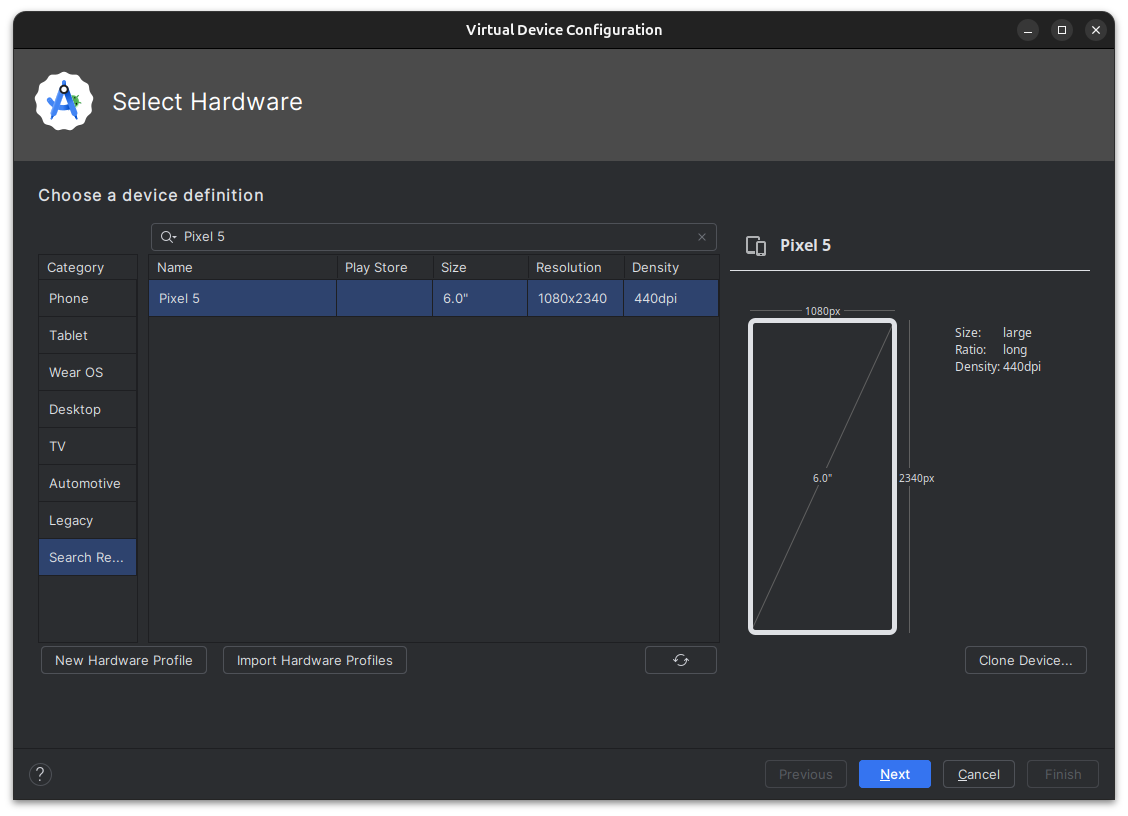
\includegraphics[width=0.75\linewidth]{graphics/studio-pixel-5.png}
        \caption{Pixel 5 device selection.}
        \label{fig:pixel-5}
    \end{figure}

    \item For the System Image, under ``Recommended'' scroll down until you see ``Pie'' with an API version of ``28.'' If it isn't downloaded already, click the download icon next to ``Pie'' and agree to the SDK license agreement to download the system image. See Figure~\ref{fig:android-system-image} to verify that the correct system image has been selected.

    \begin{figure}[!htbp]
        \centering
        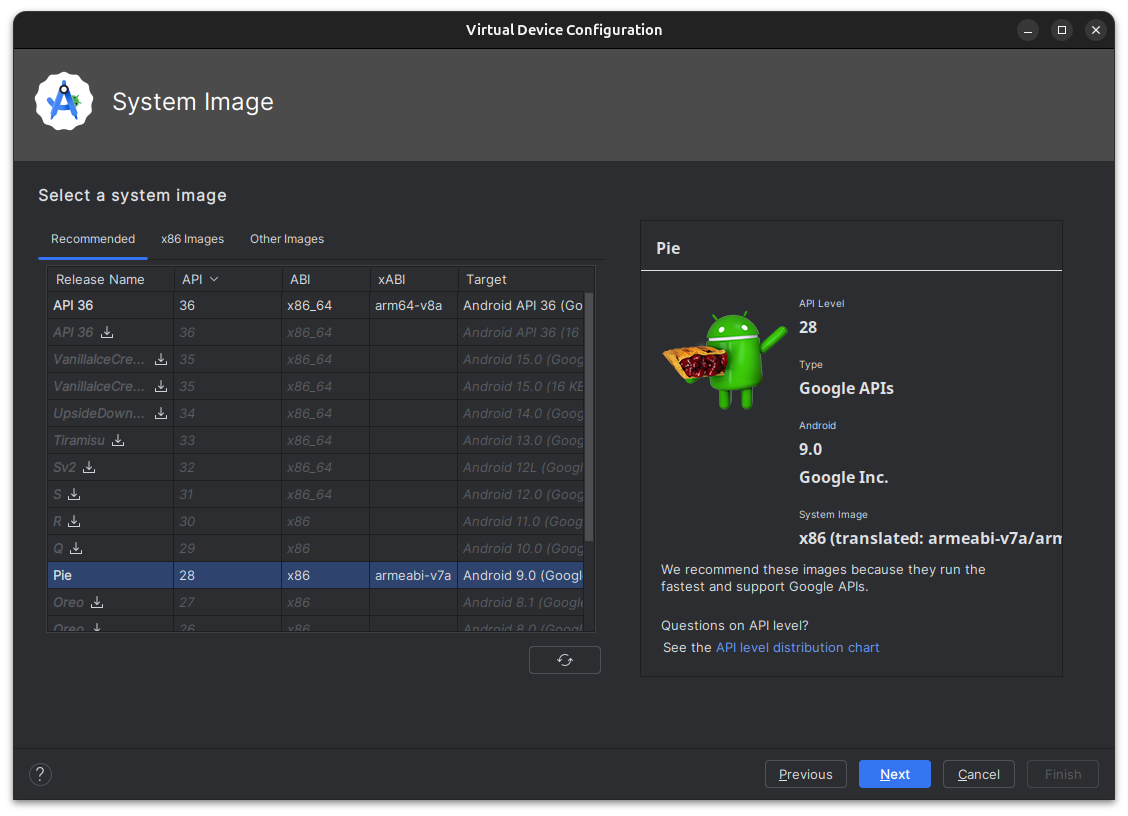
\includegraphics[width=0.75\linewidth]{graphics/studio-system-image.png}
        \caption{System Image for the Pixel 5. Ensure that Pie with API version 28 is selected.}
        \label{fig:android-system-image}
    \end{figure}
    
    \item Once downloaded, select Next then Finish before moving on to the next section.
\end{enumerate}

\newpage
\subsection*{Pre-made App Installation}
\addcontentsline{toc}{subsection}{Pre-made App Installation}

\begin{enumerate}
    \item Start the emulation device from the Device Manager (Figure~\ref{fig:start-device}). The first startup may take a few minutes.

    \begin{figure}[!htbp]
        \centering
        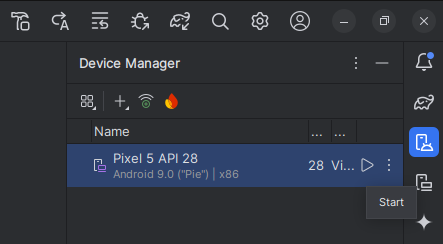
\includegraphics[width=0.75\linewidth]{graphics/studio-start-device.png}
        \caption{Starting the Pixel 5 emulator.}
        \label{fig:start-device}
    \end{figure}
    
    \item In Android Studio, along the top bar there are run configurations. Select the ``raceattack'' run configuration and run it (Figure~\ref{fig:raceattack-run-config}). Once the app opens on the Pixel 5 the process can be terminated by either closing the app on the emulator or pressing the red stop button by the run configurations.

    \begin{figure}[!htbp]
        \centering
        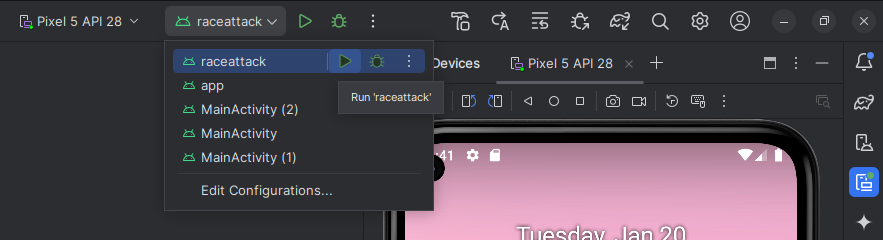
\includegraphics[width=0.75\linewidth]{graphics/studio-raceattack-run-config.png}
        \caption{Raceattack run configuration.}
        \label{fig:raceattack-run-config}
    \end{figure}

    \item Repeat the process for the previous step with the ``app'' run configuration (Figure~\ref{fig:app-run-config}).

    \begin{figure}[!htbp]
        \centering
        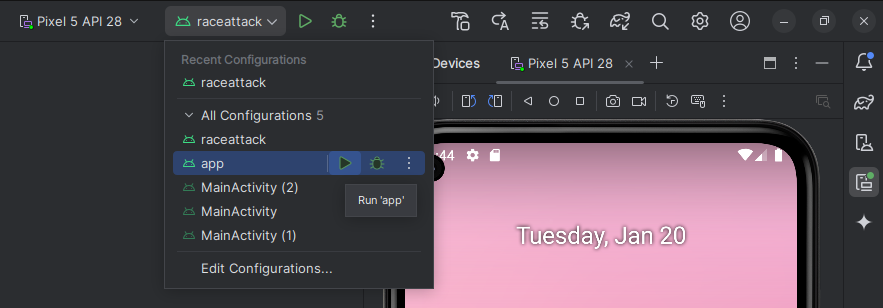
\includegraphics[width=\linewidth]{graphics/studio-app-run-config.png}
        \caption{Raceattack run configuration.}
        \label{fig:app-run-config}
    \end{figure}

    \item Once both apps are installed move on to the next section.
\end{enumerate}

\newpage
\subsection*{Fingerprint Setup}
\addcontentsline{toc}{subsection}{Fingerprint Setup}

\begin{enumerate}
    \item In the running emulation device, use your mouse to click and drag up from the home screen to open the app launcher. Open the Settings app, scroll down to the Security \& location settings, then open the Fingerprint settings. Refer to Figures~\ref{fig:settings}, \ref{fig:security}, and \ref{fig:fingerprint} for visual aides.

    \begin{figure}[!htbp]
        \centering
        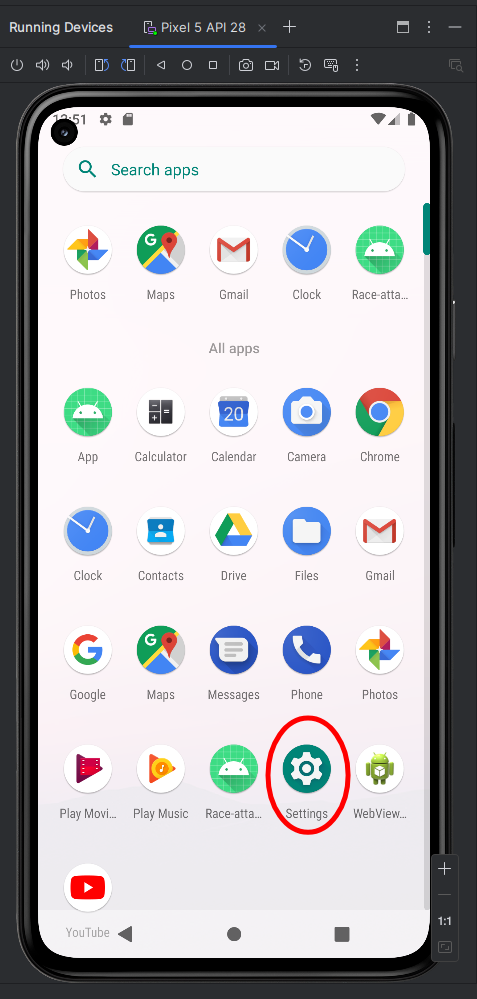
\includegraphics[width=0.5\linewidth]{graphics/studio-settings.png}
        \caption{Opening the Settings app.}
        \label{fig:settings}
    \end{figure}

    \begin{figure}[!htbp]
        \centering
        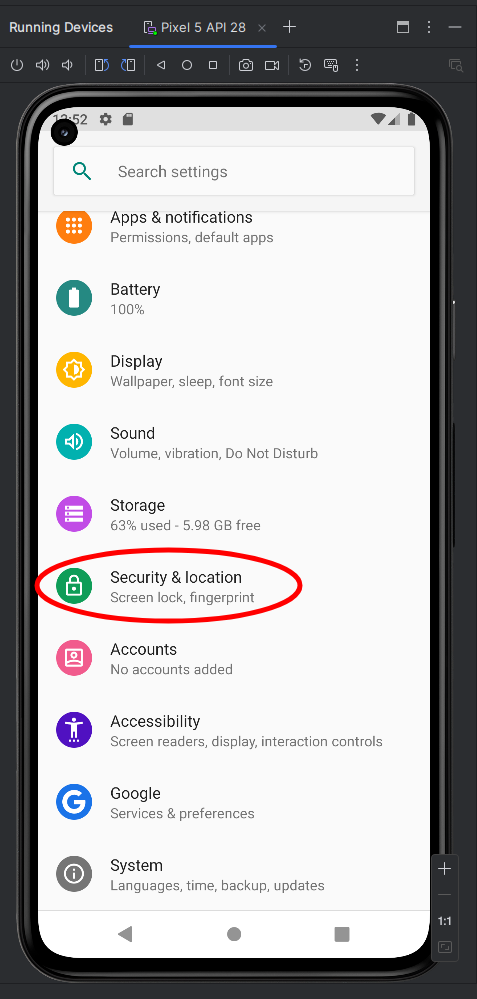
\includegraphics[width=0.65\linewidth]{graphics/studio-security-location.png}
        \caption{Opening the Security \& locations settings.}
        \label{fig:security}
    \end{figure}

    \begin{figure}[!htbp]
        \centering
        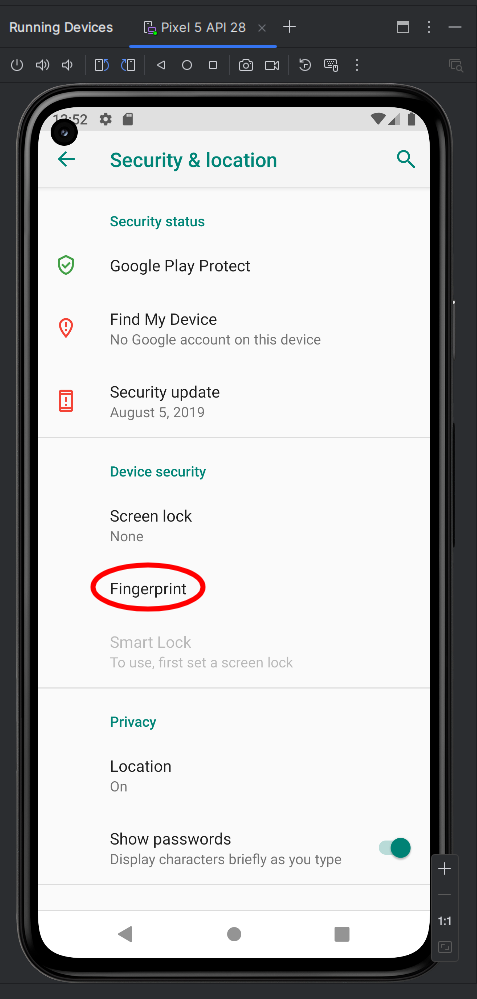
\includegraphics[width=0.65\linewidth]{graphics/studio-fingerprint.png}
        \caption{Opening the Fingerprint settings.}
        \label{fig:fingerprint}
    \end{figure}
    
    \item Choose Next, Fingerprint + Password, Yes, enter "workshop" or any other easy to remember password and select Next, re-type your password and select Confirm, select Show all notification content, Done.    
    \item To actually use the sensor, select the three dots above the emulation device (Figure~\ref{fig:ext-controls}) to open the Extended Controls menu. Select ``Fingerprint'' in the Extended Controls Menu (Figure~\ref{fig:ext-controls-fingerprint}) and then click the ``Touch Sensor'' button until the fingerprint has been added.

    \begin{figure}[!htbp]
        \centering
        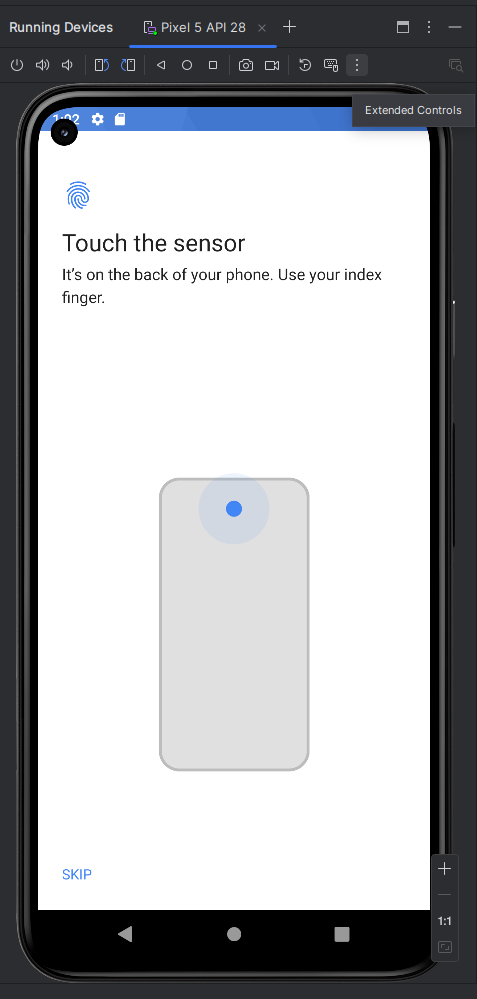
\includegraphics[width=0.65\linewidth]{graphics/studio-ext-controls.png}
        \caption{Opening the Extended Controls Menu.}
        \label{fig:ext-controls}
    \end{figure}

    \begin{figure}[!htbp]
        \centering
        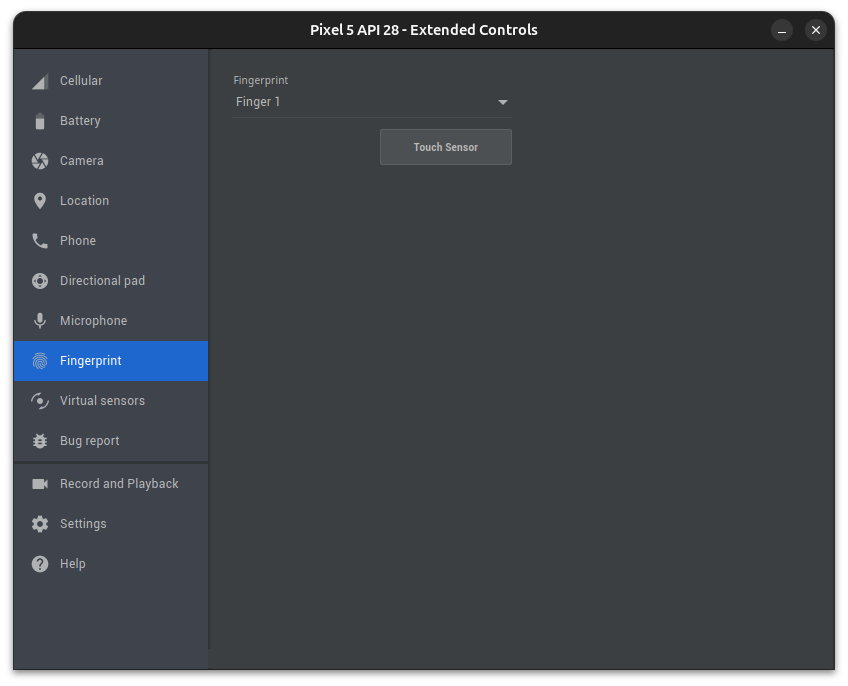
\includegraphics[width=\linewidth]{graphics/studio-ext-controls-fingerprint.png}
        \caption{Opening the Fingerprint control menu.}
        \label{fig:ext-controls-fingerprint}
    \end{figure}
    
    \item Congratulations, you've successfully set up Android Studio for this workshop and are now ready for the Mobile Security workshop segment of the BEACON Labs Workshop. Thank you for coming prepared! If you haven't already, please follow the instructions for the Web and Network Security material setups. We look forward to seeing you in Boise for the workshop!
\end{enumerate}

\end{document}

%%%%%%%%%%%%%%%%%%%%%%%%%%%%%%%%%%%%%%%%%